\documentclass[aspectratio=169,usenames,dvipsnames]{beamer}

% fonts
%\usepackage[T1]{fontenc}
%\usepackage[utf8]{inputenc}

%\usefonttheme{professionalfonts} % using non standard fonts for beamer
\usefonttheme{serif} % default family is serif

\usepackage{palatino}
%\usepackage{gfsartemisia}
%\usepackage{theanooldstyle}

\usepackage{euscript}	 % Шрифт Евклид
\usepackage{mathrsfs} % Красивый матшрифт
\usepackage{amssymb}
\usepackage{bm}
\usepackage{calc} % perform arithmetic on the arguments
\usepackage{cancel} % cancelling things
\usepackage{marvosym} % fancy arrow
\usepackage[ruled,vlined]{algorithm2e}
\usepackage{algorithmic}

\definecolor{mygreen}{HTML}{348A41}  % 53945D
\definecolor{myred}{HTML}{B73239} 
\definecolor{myorange}{HTML}{AB5F1F}  % 805129
\definecolor{mypurple}{HTML}{533E8F} 
\definecolor{myblack}{HTML}{4C4848} 
\definecolor{mygrey}{HTML}{F4EDE0} %  F5F1EA

\usepackage{epstopdf}
\usepackage{xcolor}

% adding images
\usepackage{graphicx} 
\usepackage{tcolorbox}

% adding gifs
\usepackage{animate}

% positioning textblocks
\usepackage[absolute, overlay]{textpos} 
\textblockorigin{0mm}{0mm} % start everything near the top-left corner

% Работа с русским языком
\usepackage{cmap}					% поиск в PDF
%\usepackage{mathtext} 				% русские буквы в фомулах
%\usepackage[T2A]{fontenc}			% кодировка
%\usepackage[utf8]{inputenc}			% кодировка исходного текста

% Дополнительная работа с математикой
%\usepackage{amsmath,amsfonts,amssymb,amsthm,mathtools} % AMS
%\usepackage{icomma} % "Умная" запятая: $0,2$ --- число, $0, 2$ --- перечисление

%% Номера формул
%\mathtoolsset{showonlyrefs=true} % Показывать номера только у тех формул, на которые есть \eqref{} в тексте.

% Работа с картинками
\usepackage{graphicx}  % Для вставки рисунков
\graphicspath{{images/}}  % папки с картинками
\usepackage{wrapfig} % Обтекание рисунков и таблиц текстом

% drawing with tikz
\usepackage{tikz}
\usepackage{hf-tikz}
\usetikzlibrary{arrows}
\usetikzlibrary{shapes}
\usetikzlibrary{plotmarks}

\tikzset{
	treenode/.style = {align=center, inner sep=1.ex, minimum size=1cm,
		font=\sffamily},
	arn_n/.style = {treenode, rectangle, black, draw=black, minimum width = 0.05\textwidth, minimum height = 1 cm},% 
	level distance = 2.5cm,
	level 1/.style={sibling distance=16.cm},
	level 2/.style={sibling distance=8.cm},
	level 3/.style={sibling distance=3.7cm}
}

  \tikzset{
	invisible/.style={opacity=0},
	visible on/.style={alt=#1{}{invisible}},
	alt/.code args={<#1>#2#3}{%
		\alt<#1>{\pgfkeysalso{#2}}{\pgfkeysalso{#3}} % \pgfkeysalso doesn't change the path
	},
}

%% Работа с таблицами
%\usepackage{array,tabularx,tabulary,booktabs} % Дополнительная работа с таблицами
%\usepackage{longtable}  % Длинные таблицы
%\usepackage{multirow} % Слияние строк в таблице
%\renewcommand{\arraystretch}{1.3} %The height of each row is set to 1.5 relative to its default height. 

% Two ways of getting rid of total slides number

%\setbeamertemplate{footline}
%    {\begin{beamercolorbox}[sep=1ex]{author in head/foot}
%      \rlap{\textit{\insertshorttitle}}\hfill\insertauthor\hfill\llap{\insertframenumber}%
%      \end{beamercolorbox}%
%}

\makeatletter
\setbeamertemplate{footline}
{
	\leavevmode%
	\hbox{%
		\begin{beamercolorbox}[wd=.333333\paperwidth,ht=2.25ex,dp=1ex,center]{author in head/foot}%
		Olga Razuvaeva, ITEP and MEPhI
%			\usebeamerfont{author in head/foot}
%			\insertshortauthor~~\beamer@ifempty{\insertshortinstitute}{}{(\insertshortinstitute)}
		\end{beamercolorbox}%
		\begin{beamercolorbox}[wd=.333333\paperwidth,ht=2.25ex,dp=1ex,center]{title in head/foot}%
		Introduction to ANN
%			\usebeamerfont{title in head/foot}\insertshorttitle
		\end{beamercolorbox}%
		\begin{beamercolorbox}[wd=.333333\paperwidth,ht=2.25ex,dp=1ex,right]{date in head/foot}%
			\usebeamerfont{date in head/foot}\insertshortdate\hspace*{2em}
			\insertframenumber/\inserttotalframenumber\hspace*{2ex} 
	\end{beamercolorbox}}%
	\vskip0pt%
}
\makeatother

% Beamer presentation style
\mode<presentation> {
	\usetheme{Pittsburgh}
	\usecolortheme{dove}
	%\setbeamertemplate{footline} % To remove the footer line in all slides uncomment this line
	%\setbeamertemplate{footline}[page number] % To replace the footer line in all slides with a simple slide count uncomment this line
	%\setbeamertemplate{navigation symbols}{} % To remove the navigation symbols from the bottom of all slides uncomment this line
	
	%	\setbeamercolor{frametitle}{fg=white,bg=greyone}
	%	\setbeamercolor{titlelike}{parent=palette quaternary}
	
	%	\setbeamertemplate{frametitle}
	%	{
	%		\begin{textblock*}{\hsize}(.75\hsize,0.05\vsize)
	%			\begin{tcolorbox}[colframe=white, colback=mygrey, width=0.33\hsize,
	%				arc=2.mm, boxsep=2mm,
	%				box align=center,
	%				halign=center,
	%				valign=center,
	%				]
	%				\insertframetitle
	%			\end{tcolorbox}
	%		\end{textblock*}
	%	}
}

%% custom title
%\newcommand{\myframetitle}[3]{
%	\begin{textblock*}{\hsize}(#1,0.05\vsize)
%		\begin{tcolorbox}[colframe=white, colback=mygrey, width=#2,
%			arc=2.mm, boxsep=2mm,
%			box align=center,
%			halign=center,
%			valign=center,
%			]
%			\Large
%			#3
%		\end{tcolorbox}
%	\end{textblock*}
%}

% custom title
\newcommand{\myframetitle}[3]{
	\begin{textblock*}{#1}(#2,0.05\vsize)
		\begin{tcolorbox}[colframe=white, colback=mygrey, width=#1,
			arc=2.mm, boxsep=2mm,
			box align=center,
			halign=center,
			valign=center,
			]
			\Large
			\centering
			#3
		\end{tcolorbox}
	\end{textblock*}
}

% custom subtitle
\newcommand{\myframesubtitle}[2]{
	
	\begin{textblock*}{5cm}(#1,0.123\vsize)
		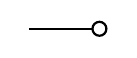
\begin{tikzpicture}
		\draw[thick,-o,black] (0.,0.) -- (1.0,0.);
		\end{tikzpicture}
	\end{textblock*}
	
	\begin{textblock*}{0.5\hsize}(#1+0.075\paperwidth,0.1\vsize)
		\normalsize
		\vspace{0.6mm}
		%		\centering
		#2
	\end{textblock*}
}

% new color for the bullet/subbullet
\newcommand{\mybullet}{$\textcolor{myblack}{\bullet}$}
\newcommand{\mysubbullet}{$\textcolor{myblack}{\circ}$}
\newcommand{\ev}{\mathbb{E}_{\text{p}(\bm x,y)}}
\newcommand{\pluseq}{\mathrel{+}=}

%\title{Introduction to Machine Learning\\
%Lecture 1}
%\author[name]{Oleg Filatov \inst{1} \and   Zakharov \inst{2}}%
%\institute{
%	\inst{1} DESY 
%	\inst{2} Novosibirsk State University
%	\newline
%	\vspace{1em}
%	
%%	\includegraphics[width=1.1cm]{CMS_logo.pdf}\hspace*{0.4cm}
%	\includegraphics[width=1.1cm]{DESY_logo.png}\hspace*{0.4cm}
%	\includegraphics[width=2.1cm]{NSU_logo.png}\hspace*{0.4cm}
%}
%
%\date{}

%----------------------------------------------------------------------------------------
%	TITLE PAGE
%----------------------------------------------------------------------------------------

\author[Olga Razuvaeva]{Olga Razuvaeva\inst{1, 2}, Sergey Korpachev\inst{3, 4} and Stepan Zakharov\inst{5}}%
\institute{
    \newline
	\inst{1} {Institute for Theoretical and Experimental Physics}\\
	\inst{2} {National Research Nuclear University MEPhI (Moscow Engineering Physics Institute)}\\
	\inst{3} {Moscow Institute of Physics and Technology}\\
	\inst{4} {Lebedev Physical Institute of the Russian Academy of Sciences}\\
	\inst{5} {Novosibirsk State University}\\
	}
\titlegraphic{
	%\vspace{-.5cm}
	%\hspace{1cm}
	\includegraphics[width=1.5cm]{itep_logo.png}\hspace*{0.5cm}
	\includegraphics[width=1.5cm]{mephi_logo.jpg}\hspace*{0.1cm}
	\includegraphics[width=2.5cm]{mipt_logo.png}\hspace*{0.1cm}
	\includegraphics[width=1.5cm]{lpi_logo.png}\hspace*{0.6cm}
	\includegraphics[width=3.0cm]{nsu_logo.png}\hspace*{0.3cm}
}
\date[November 22, 2020]{}

%------------------------------------------------

\begin{document}

\begin{frame}
    \centering
    \huge
    %\vspace{-0.3\paperheight}
    \begin{tcolorbox}[colframe=white, colback=mygrey, width=0.5\paperwidth,
    	arc=2.mm, boxsep=2mm,
    	box align=center,
    	halign=center,
    	valign=center,
    	]
    	\Large
    	Artificial neural networks
    \end{tcolorbox}
    \vspace{0.1\paperheight}
    \centering
    \large
    \insertauthor\\
    \footnotesize
    \vspace{0.03\paperheight}
    \hspace{0.17\paperwidth}
    \insertinstitute
    \vfill
    \inserttitlegraphic
    \transfade[duration=.4]
\end{frame}

%------------------------------------------------

\begin{frame}[t]
	\myframetitle{0.2\paperwidth}{0.04\paperwidth}{?????Outline?????}
	\vspace{0.2\paperheight}
	\begin{itemize}
	    \centering
		\itemsep0.8ex
		\setbeamertemplate{items}{\mybullet}
    	\item {Non-linearity in data}
    	\item {Feature extraction}
    	\item {ANN structure}
	    \item {How to train?}
	    \item [\textcolor{blue}{\textbullet}] {\textcolor{blue} {Deep Learning}}
	    \item {The Achilles heel of the DL models}
	    \item {Evolution of GD}
	    \item {Reaching stability}
	    \item {Network architectures}
	\end{itemize}
\transfade[duration=.4]
\end{frame}

%------------------------------------------------
%------------------------------------------------
\section{Modelling nonlinearities}
%------------------------------------------------
%------------------------------------------------

\begin{frame}[plain]
    \centering
    \huge
    %\begin{textblock*}{0.3\paperwidth}(0.25\paperwidth,0.3\paperheight)
    \centering
    \vspace{0.1\paperheight}
    \begin{tcolorbox}[colframe=white, colback=mygrey, width=0.4\paperwidth,
    	arc=2.mm, boxsep=2mm,
    	box align=center,
    	halign=center,
    	valign=center,
    	]
    	\insertsection
    \end{tcolorbox}
    %\end{textblock*}
    \transfade[duration=.4]
\end{frame}

%------------------------------------------------

\subsection{they exist}
\begin{frame}
    \myframetitle{0.45\paperwidth}{0.04\paperwidth}{\insertsection}
    \myframesubtitle{0.47\paperwidth}{\insertsubsection}
    \centering
	\vspace{1.5cm}
	\includegraphics[width=0.8\linewidth]{lin_nonlin.png}\\
	Do you know how to describe the non-linear data in the right picture?\\
	Linear model, seriously?\\
	!!!!!\textcolor{red}{Here goes picture of linear vs non-linear data}!!!!!
\end{frame}

%------------------------------------------------

\subsection{linear models}
\begin{frame}
    \myframetitle{0.45\paperwidth}{0.04\paperwidth}{\insertsection}
    \myframesubtitle{0.47\paperwidth}{\insertsubsection}
    \vspace{1.5cm}
    \begin{itemize}
        \item {The linear model does not describe complex nonlinear data}
        \item {A combination of linear models is also a linear model}
    \end{itemize}
    !!!!!\textcolor{red}{Explanation why linear models don’t fit them out-of-the box}!!!!!
\end{frame}

%------------------------------------------------

\subsection{trees}
\begin{frame}
    \myframetitle{0.45\paperwidth}{0.04\paperwidth}{\insertsection}
    \myframesubtitle{0.47\paperwidth}{\insertsubsection}
    \vspace{1.5cm}
    \begin{itemize}
        \item {Trees were designed to approximate nonlinearities}
        \item {They do a pretty good job in it}
        \item {They are fast and interpretable}
        \item {But they are just "brute-force" algorithms}
        \item {They don't infer symmetries in data by design}
        \item {ad-hoc, cut-based and piecewise approximations of data at hand}
        \item {Hence, not differentiable and smooth}
    \end{itemize}
\end{frame}

%------------------------------------------------

\subsection{feature engineering}
\begin{frame}
    \myframetitle{0.45\paperwidth}{0.04\paperwidth}{\insertsection}
    \myframesubtitle{0.47\paperwidth}{\insertsubsection}
    \centering
    \vspace{1.7cm}
    \includegraphics[width=0.5\linewidth]{images/feature_engin.png}\\
    \begin{itemize}
        \item {But sometimes we know \textit{a priori} that there are transformations simplifying the problem for our model}
        \item {So that even linear models can do the job}
        \item {But this \textbf{feature engineering} is non-trivial, requires domain knowledge and is time-consuming}
    \end{itemize}
    \textbf{What if we design a model which could automatically feature-engineer itself?}
\end{frame}

%------------------------------------------------
%------------------------------------------------
\section{Neural Network}
%------------------------------------------------
%------------------------------------------------

\begin{frame}[plain]
    \centering
    \huge
    %\begin{textblock*}{0.3\paperwidth}(0.25\paperwidth,0.3\paperheight)
    \centering
    \vspace{0.1\paperheight}
    \begin{tcolorbox}[colframe=white, colback=mygrey, width=0.4\paperwidth,
    	arc=2.mm, boxsep=2mm,
    	box align=center,
    	halign=center,
    	valign=center,
    	]
    	Building the beast
    \end{tcolorbox}
    %\end{textblock*}
    \transfade[duration=.4]
\end{frame}

%------------------------------------------------

\subsection{automating FE}
\begin{frame}
    \myframetitle{0.45\paperwidth}{0.04\paperwidth}{\insertsection}
    \myframesubtitle{0.47\paperwidth}{\insertsubsection}
    \centering
    \vspace{1.7cm}
    \includegraphics[width=1.0\linewidth]{images/some_model.png}
\end{frame}

%------------------------------------------------

\begin{frame}
    \myframetitle{0.45\paperwidth}{0.04\paperwidth}{\insertsection}
    \myframesubtitle{0.47\paperwidth}{\insertsubsection}
    \centering
    \vspace{1.7cm}
    \includegraphics[width=1.0\linewidth]{images/lin_model.png}\\
    $\hat{y} = w^{T} \cdot \tilde{x} = w^{T} \cdot (W \cdot x) = (w^{T} \cdot W) \cdot x = w'^{T} \cdot x \Rightarrow$ it is still a linear model
\end{frame}

%------------------------------------------------

\begin{frame}
    \myframetitle{0.45\paperwidth}{0.04\paperwidth}{\insertsection}
    \myframesubtitle{0.47\paperwidth}{\insertsubsection}
    \centering
    \vspace{1.7cm}
    \includegraphics[width=1.0\linewidth]{images/add_nonlin.png}
    $\hat{y} = w^{T} \cdot \tilde{x} = w^{T} \cdot g(W \cdot x)$,\\
    where $g(\cdot)$ some nonlinear scalar function (applied elementwise)
\end{frame}

%------------------------------------------------

\begin{frame}
    \myframetitle{0.45\paperwidth}{0.04\paperwidth}{\insertsection}
    \myframesubtitle{0.47\paperwidth}{\insertsubsection}
    adding nonlinearity\\
    <pic from slide 12 mlhep>\\
\end{frame}

%\begin{frame}[plain]
%\centering
%\huge
%
%%\begin{textblock*}{0.3\paperwidth}(0.25\paperwidth,0.3\paperheight)
%\centering
%\vspace{0.1\paperheight}
%\begin{tcolorbox}[colframe=white, colback=mygrey, width=0.4\paperwidth,
%	arc=2.mm, boxsep=2mm,
%	box align=center,
%	halign=center,
%	valign=center,
%	]
%	\insertsection
%\end{tcolorbox}
%
%%\end{textblock*}
%
%\transfade[duration=.4]
%\end{frame}

%------------------------------------------------

\subsection{architecture}
\begin{frame}
    \myframetitle{0.45\paperwidth}{0.04\paperwidth}{\insertsection}
    \myframesubtitle{0.47\paperwidth}{\insertsubsection}
    \centering
    \vspace{1.7cm}
    \includegraphics[width=1.0\linewidth]{images/nn_details.png}\\
    $\hat{y} = w^{T} \cdot \tilde{x} = w^{T} \cdot g(W \cdot x) = \sum\limits_{j=1}\big[ w_{j} \cdot g(\sum\limits_{i}W_{ji} \cdot x_{i}) \big]$
\end{frame}

%------------------------------------------------

\subsection{terminology}
\begin{frame}
    \myframetitle{0.45\paperwidth}{0.04\paperwidth}{\insertsection}
    \myframesubtitle{0.47\paperwidth}{\insertsubsection}
    \centering
    \vspace{1.7cm}
    \begin{columns}[T]
	    \column{0.5\textwidth}
	    \begin{minipage}[t]{\linewidth}
	       \begin{center}
	           \vspace{1cm}
	           \textbf{Feed-forward network:}\\
	           \hfill \break
	           \includegraphics[width=1.0\linewidth]{images/nn_terminology.png}
            \end{center}
        \end{minipage}
	    \column{0.5\textwidth}
        \begin{minipage}[t]{\linewidth}
            \begin{itemize}
                \item {\textcolor{red}{red} nodes (vertices) $x_{1}, x_{2}, ..., x_{d}$ - features from an input layer of the ANN}
                \item {\textcolor{green}{green} nodes (vertices) - neurons from a hidden layer of the ANN}
                \item {\textcolor{blue}{blue} node (vertex) $\hat{y}$ - neuron from a output layer of the ANN}
                \item {Straight lines (edges) correspond to weights ($w$) between neurons}
                \item {$g(\cdot)$ - nonlinear activation function, for example, a sigmoid function}
                \item {Each layer (except the output layer) has a bias neuron: $x_{bias} = 1$}
            \end{itemize}
        \end{minipage}
    \end{columns}
\end{frame}

%------------------------------------------------

\subsection{human brain}
\begin{frame}
    \myframetitle{0.45\paperwidth}{0.04\paperwidth}{\insertsection}
    \myframesubtitle{0.47\paperwidth}{\insertsubsection}
    \centering
    \vspace{1.7cm}
	It follows the way of human brain processing. ANN modelled how a neuron works in the human brain.\\
	\includegraphics[width=0.9\linewidth]{brain.png}
    Neurons on human brain consist of a nucleus, dendrites, cell body, and axon. The number of neurons in humans is approximately 140 billion, consist of 100 billion neurons and 40 billion synapses in neurons.
\end{frame}

%------------------------------------------------
%------------------------------------------------
\section{Training}
%------------------------------------------------
%------------------------------------------------

\begin{frame}[plain]
    \centering
    \huge
    %\begin{textblock*}{0.3\paperwidth}(0.25\paperwidth,0.3\paperheight)
    \centering
    \vspace{0.1\paperheight}
    \begin{tcolorbox}[colframe=white, colback=mygrey, width=0.4\paperwidth,
    	arc=2.mm, boxsep=2mm,
    	box align=center,
    	halign=center,
    	valign=center,
    	]
    	Training the beast
    \end{tcolorbox}
    %\end{textblock*}
    \transfade[duration=.4]
\end{frame}

%------------------------------------------------

\subsection{how to train?}
\begin{frame}
    \myframetitle{0.45\paperwidth}{0.04\paperwidth}{\insertsection}
    \myframesubtitle{0.47\paperwidth}{\insertsubsection}
    \vspace{1.5cm}
    \begin{itemize}
        \item {NN is basically a composite linear model (with nonlinearities)}
        \item {We can use gradient descent (GD) to train}
        \item {GD algorithm:\\
        $\theta_{i+1} = \theta_{i} - \eta \cdot \textcolor{red}{\nabla Q (\theta_{i})}$}
        \item {Do you know how to calculate the gradient of the weights?}
    \end{itemize}
\end{frame}

%------------------------------------------------

\subsection{chain rule}
\begin{frame}
    \myframetitle{0.45\paperwidth}{0.04\paperwidth}{\insertsection}
    \myframesubtitle{0.47\paperwidth}{\insertsubsection}
    \vspace{1.5cm}
    \begin{itemize}
        \item {But gradients are hard to derive analytically}
        \item {Writing down (into NN framework) all the derivatives is tough}
        \item {The approach doesn't generalize to architectures}
        \item {But NN is just a composite model $\Rightarrow$ can use chain rule for differentiating it}
    \end{itemize}
\end{frame}

%------------------------------------------------

\subsection{chain rule: examples}
\begin{frame}
    \myframetitle{0.45\paperwidth}{0.04\paperwidth}{\insertsection}
    \myframesubtitle{0.47\paperwidth}{\insertsubsection}
    \vspace{1.5cm}
	\centering
	\begin{itemize}
    	\centering
	    \item We know how to find the derivative of a simple function.
	    \item Let's remember the rule for differentiating complex functions.
	\end{itemize}
	$\cfrac{\partial f \big(t(x) \big) }{\partial x} = \cfrac{\partial f(t)}{\partial t(x)} \cdot \cfrac{\partial t(x)}{\partial x}$
	\begin{itemize}
	    \centering
    	\item What is the derivative of following function with respect to $x$: $\color{blue} {sin(x^2 + 5)}$?
    	\item What is the derivative of the sigmoid function?
	\end{itemize}
    Can you convert it to $\sigma'(x) = f \big( \sigma(x) \big)$?\\
	\begin{itemize}
	    \centering
	    \item Sigmoid function: $\sigma(x) = \cfrac{1}{1+e^{-x}}$
	\end{itemize}
	\hfill \break
	\onslide<2-> \color{red} {Answer:} $\sigma'(x) = \sigma(x) \cdot \big( 1 - \sigma(x) \big)$
\end{frame}

%------------------------------------------------

\subsection{weights update}
\begin{frame}
    \myframetitle{0.45\paperwidth}{0.04\paperwidth}{\insertsection}
    \myframesubtitle{0.47\paperwidth}{\insertsubsection}
    \centering
    \vspace{1.7cm}
    \includegraphics[width=0.5\linewidth]{images/train_1.png}\\
    !!!!!\textcolor{red}{also mention forward and backward passes}!!!!!\\
    !!!!!\textcolor{red}{maybe it's worth to also put ML in HEP slide first to show the general idea}!!!!!
\end{frame}

%------------------------------------------------

\subsection{weights update}
\begin{frame}
    \myframetitle{0.45\paperwidth}{0.04\paperwidth}{\insertsection}
    \myframesubtitle{0.47\paperwidth}{\insertsubsection}
    \centering
    \vspace{1.7cm}
    \textbf{Consider a simpler neural network}\\
    \includegraphics[width=0.8\linewidth]{images/train_2.png}\\
\end{frame}

%------------------------------------------------

\subsection{weights update}
\begin{frame}
    \myframetitle{0.45\paperwidth}{0.04\paperwidth}{\insertsection}
    \myframesubtitle{0.47\paperwidth}{\insertsubsection}
    \centering
    \vspace{1.7cm}
    \includegraphics[width=0.8\linewidth]{images/train_3.png}\\
\end{frame}

%------------------------------------------------

\subsection{back propagation}
\begin{frame}
    \myframetitle{0.45\paperwidth}{0.04\paperwidth}{\insertsection}
    \myframesubtitle{0.47\paperwidth}{\insertsubsection}
    \centering
    \vspace{1.7cm}
    \includegraphics[width=0.8\linewidth]{images/train_4.png}\\
\end{frame}

%------------------------------------------------

\subsection{back propagation}
\begin{frame}
    \myframetitle{0.45\paperwidth}{0.04\paperwidth}{\insertsection}
    \myframesubtitle{0.47\paperwidth}{\insertsubsection}
    \centering
    \vspace{1.7cm}
    \includegraphics[width=0.8\linewidth]{images/train_5.png}\\
\end{frame}

%------------------------------------------------

\subsection{back propagation}
\begin{frame}
    \myframetitle{0.45\paperwidth}{0.04\paperwidth}{\insertsection}
    \myframesubtitle{0.47\paperwidth}{\insertsubsection}
    \centering
    \vspace{1.7cm}
    \includegraphics[width=0.8\linewidth]{images/train_6.png}\\
\end{frame}

%------------------------------------------------

\subsection{back propagation}
\begin{frame}
    \myframetitle{0.45\paperwidth}{0.04\paperwidth}{\insertsection}
    \myframesubtitle{0.47\paperwidth}{\insertsubsection}
    \centering
    \vspace{1.7cm}
    \includegraphics[width=0.8\linewidth]{images/train_7.png}\\
\end{frame}

%------------------------------------------------

\subsection{back propagation}
\begin{frame}
    \myframetitle{0.45\paperwidth}{0.04\paperwidth}{\insertsection}
    \myframesubtitle{0.47\paperwidth}{\insertsubsection}
    \centering
    \vspace{1.7cm}
    \includegraphics[width=0.8\linewidth]{images/train_8.png}\\
\end{frame}

%------------------------------------------------

\subsection{forward pass}
\begin{frame}
    \myframetitle{0.45\paperwidth}{0.04\paperwidth}{\insertsection}
    \myframesubtitle{0.47\paperwidth}{\insertsubsection}
    \centering
    \vspace{1.7cm}
    \includegraphics[width=0.8\linewidth]{images/train_9.png}\\
\end{frame}

%------------------------------------------------

\subsection{backward pass}
\begin{frame}
    \myframetitle{0.45\paperwidth}{0.04\paperwidth}{\insertsection}
    \myframesubtitle{0.47\paperwidth}{\insertsubsection}
    \centering
    \vspace{1.7cm}
    \includegraphics[width=0.8\linewidth]{images/train_10.png}\\
\end{frame}

%------------------------------------------------
%------------------------------------------------
\section{Break time}
%------------------------------------------------
%------------------------------------------------

\begin{frame}[plain]
    \centering
    \huge
    %\begin{textblock*}{0.3\paperwidth}(0.25\paperwidth,0.3\paperheight)
    \centering
    \vspace{0.1\paperheight}
    \begin{tcolorbox}[colframe=white, colback=mygrey, width=0.4\paperwidth,
    	arc=2.mm, boxsep=2mm,
    	box align=center,
    	halign=center,
    	valign=center,
    	]
    	\insertsection
    \end{tcolorbox}
    %\end{textblock*}
    \transfade[duration=.4]
\end{frame}

%------------------------------------------------

\subsection{this is big brain time}
\begin{frame}
    \myframetitle{0.45\paperwidth}{0.04\paperwidth}{\insertsection}
    \myframesubtitle{0.47\paperwidth}{\insertsubsection}
    \vspace{1.5cm}
	\centering
    \includegraphics[width=0.35\linewidth]{big_brain_time.jpg}\\
    \begin{itemize}
    	\centering
	    \item Is it necessary to use a bias neuron? Why?
	    \item What values can the weights of neurons take?
	\end{itemize}
\end{frame}

%------------------------------------------------
%------------------------------------------------
\section{Going deeper}
%------------------------------------------------
%------------------------------------------------

\begin{frame}[plain]
\centering
\huge

%\begin{textblock*}{0.3\paperwidth}(0.25\paperwidth,0.3\paperheight)
\centering
\vspace{0.1\paperheight}
\begin{tcolorbox}[colframe=white, colback=mygrey, width=0.4\paperwidth,
	arc=2.mm, boxsep=2mm,
	box align=center,
	halign=center,
	valign=center,
	]
	\insertsection
\end{tcolorbox}

%\end{textblock*}

\transfade[duration=.4]
\end{frame}

%------------------------------------------------

\subsection{Universal approximation theorem }
\begin{frame}

\myframetitle{0.45\paperwidth}{0.04\paperwidth}{\insertsection}
\myframesubtitle{0.47\paperwidth}{\insertsubsection}

\end{frame}

\subsection{stack more layers}
\begin{frame}

\myframetitle{0.45\paperwidth}{0.04\paperwidth}{\insertsection}
\myframesubtitle{0.47\paperwidth}{\insertsubsection}

in practise stacking more layers improves performance\\
also example of Stepan with human brain (slide 18)\\


\end{frame}
%------------------------------------------------

\subsection{problems}
\begin{frame}

\myframetitle{0.45\paperwidth}{0.04\paperwidth}{\insertsection}
\myframesubtitle{0.47\paperwidth}{\insertsubsection}

slide explaining vanishing gradients

\end{frame}

%------------------------------------------------

\begin{frame}

\myframetitle{0.45\paperwidth}{0.04\paperwidth}{\insertsection}
\myframesubtitle{0.47\paperwidth}{\insertsubsection}

slide explaining exploding gradients

\end{frame}

%------------------------------------------------

\begin{frame}

\myframetitle{0.45\paperwidth}{0.04\paperwidth}{\insertsection}
\myframesubtitle{0.47\paperwidth}{\insertsubsection}

slide explaining vanishing gradients

\end{frame}

%------------------------------------------------
%------------------------------------------------
\section{Activation functions}
%------------------------------------------------
%------------------------------------------------

\subsection{}
\begin{frame}

\myframetitle{0.45\paperwidth}{0.04\paperwidth}{\insertsection}
\myframesubtitle{0.47\paperwidth}{\insertsubsection}

solution: improve activation function
slides for that with examples

\end{frame}
%------------------------------------------------


%------------------------------------------------
%------------------------------------------------
\section{Weight init schemas}
%------------------------------------------------
%------------------------------------------------

\subsection{}
\begin{frame}

\myframetitle{0.45\paperwidth}{0.04\paperwidth}{\insertsection}
\myframesubtitle{0.47\paperwidth}{\insertsubsection}

solutions: proper weight initialization
slides for that with examples

\end{frame}


%------------------------------------------------
%------------------------------------------------
\section{Modifying gradient descent}
%------------------------------------------------
%------------------------------------------------

\subsection{complexity}
\begin{frame}

\myframetitle{0.45\paperwidth}{0.04\paperwidth}{\insertsection}
\myframesubtitle{0.47\paperwidth}{\insertsubsection}

complicated model -> complicated landscape -> easy to stuck in local minumum  \\
slide showing loss landscape and emphasizing the problem\\
then slides with modifications of SGD

\end{frame}

%------------------------------------------------

\subsection{classical SGD}
\begin{frame}

\myframetitle{0.45\paperwidth}{0.04\paperwidth}{\insertsection}
\myframesubtitle{0.47\paperwidth}{\insertsubsection}

\end{frame}

%------------------------------------------------

\subsection{Momentum/Nesterov}
\begin{frame}

\myframetitle{0.45\paperwidth}{0.04\paperwidth}{\insertsection}
\myframesubtitle{0.47\paperwidth}{\insertsubsection}

\end{frame}

%------------------------------------------------

\subsection{Adagrad/RMSProp/Adam}
\begin{frame}

\myframetitle{0.45\paperwidth}{0.04\paperwidth}{\insertsection}
\myframesubtitle{0.47\paperwidth}{\insertsubsection}

\end{frame}

%------------------------------------------------
%------------------------------------------------
\section{Tackling overfitting}
%------------------------------------------------
%------------------------------------------------

\subsection{complexity}
\begin{frame}

\myframetitle{0.45\paperwidth}{0.04\paperwidth}{\insertsection}
\myframesubtitle{0.47\paperwidth}{\insertsubsection}

highly complex models -> prone to overfitting\\
some pics, maybe loss landscape once again
\end{frame}

%------------------------------------------------

\subsection{weight regularisation}
\begin{frame}

\myframetitle{0.45\paperwidth}{0.04\paperwidth}{\insertsection}
\myframesubtitle{0.47\paperwidth}{\insertsubsection}

already know that, recap slide
\end{frame}

%------------------------------------------------

\subsection{dropout}
\begin{frame}

\myframetitle{0.45\paperwidth}{0.04\paperwidth}{\insertsection}
\myframesubtitle{0.47\paperwidth}{\insertsubsection}


\end{frame}

%------------------------------------------------

\subsection{batchnorm}
\begin{frame}

\myframetitle{0.45\paperwidth}{0.04\paperwidth}{\insertsection}
\myframesubtitle{0.47\paperwidth}{\insertsubsection}


\end{frame}

%------------------------------------------------

\subsection{summary}
\begin{frame}

\myframetitle{0.45\paperwidth}{0.04\paperwidth}{\insertsection}
\myframesubtitle{0.47\paperwidth}{\insertsubsection}


\end{frame}

%------------------------------------------------

\end{document}
